
%%%%%%%%OpenModelica description starts


\section{OpenModelica}
\label{sec:OpenModelica-start}
OpenModelica is a free and open source environment based on the Modelica modeling language 
for simulating, optimizing, and analyzing complex dynamic systems \cite{om-ref}.
It is a powerful tool that can be used to design and simulate complete control systems. 
% The toolbox 'OpenModelica-Arduino' enables the interfacing of Arduino with OpenModelica by calling a set of c functions from OpenModelica.   

In the upcoming sections, we have provided the steps to install OpenModelica on Windows and Linux. 
After installing OpenModelica, the readers should watch the tutorials on OpenModelica provided on 
{\tt https://spoken-tutorial.org/}. Ideally, one should go through all the tutorials labeled as Basic. 
However, we strongly recommend the readers should watch the second and third tutorials, i.e., 
{\tt Introduction to OMEdit} and {\tt Examples through OMEdit}.


\subsection{Downloading and installing on Windows} \label{openmodelica-install-windows}
This book uses Stable Development of OpenModelica 1.17.0 for demonstrating 
the experiments, both on Windows and Linux. It may be noted that 
OpenModelica requires approximately 8 GB of space for its installation. 
Starting from download, we shall go through the steps to set up OpenModelica 
1.17.0 on Windows OS:

\begin{enumerate}
      \item Visit the URL {\tt https://openmodelica.org/}.  At the top of the page, locate the Download tab. On hovering the cursor on this tab, a drop-down menu appears. In that menu, click on Windows. 
      \item From the section Download Windows, click on the binaries 1.17.0 (32bit/64bit) next to the Stable Development of OpenModelica. 
      \item A webpage named Index of /omc/builds/windows/releases/1.17/0 appears. Now, click on 32-bit or 64-bit depending on your operating system. We will continue with a 64-bit installation. 
      \item Once you select 64-bit, a webpage named Index of /omc/builds/windows/releases/1.17/0/64bit appears. You should get a list of files here. Click on the executable (.exe) file to download the binaries for OpenModelica.
      \item Locate the executable file and double-click on it to begin the 
      installation. After double-clicking on the executable file, 
      you might get an alert on your screen (something like Windows protected your PC). 
      If this happens, locate More info in this alert window and click on 
      Run Anyway, as shown in \figref{om-run-anyway} to continue with the 
      installation. All the default parameters of the installation are acceptable. 
\end{enumerate}

\begin{figure}
      \centering
      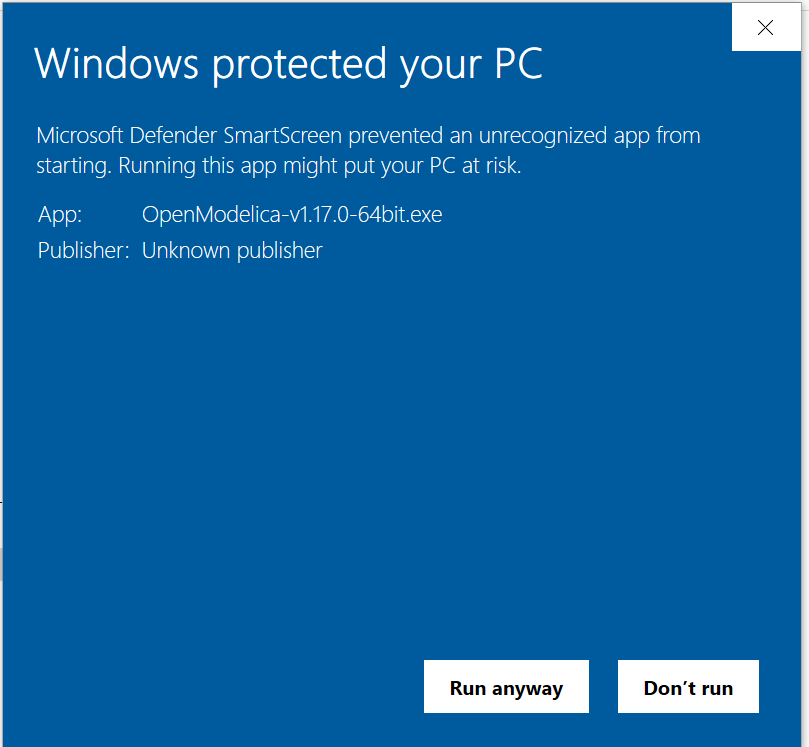
\includegraphics[width=\lgfig]{\LocSWfig/openmodelica-run-anyway.png}
      \caption{Allowing Microsoft Defender to run the executable file}
      \label{om-run-anyway}
\end{figure}

Once OpenModelica has been installed, OpenModelica Connection Editor (OMEdit) 
can be launched from the Start menu.  When you 
launch OMEdit for the first time, you might get a notification for setting up 
Modelica Standard Library version, as shown in \figref{om-help}. Here, you 
should choose the option "Load MSL v3.2.3" and click OK.  To know how to execute models 
in OMEdit, the readers are advised to refer to \secref{OpenModelica-code-execution}. 


\subsection{Downloading and installing on GNU/Linux Ubuntu} \label{openmodelica-install-linux}
On Linux, we can install OpenModelica from the terminal. The readers are advised to visit 
{\tt https://openmodelica.org/download/download-linux} and follow the instructions for installing OpenModelica.
We recommend the readers should install the latest stable version of OpenModelica. 
Once OpenModelica has been installed successfully, OpenModelica Connection Editor (OMEdit) can be launched
from the terminal. Open a terminal by pressing Alt+Ctrl+T and type OMEdit. When you 
launch OMEdit for the first time, you might get a notification for setting up 
Modelica Standard Library version, as shown in \figref{om-help}. Here, you 
should choose the option "Load MSL v3.2.3" and click OK.  
\begin{figure}
      \centering
      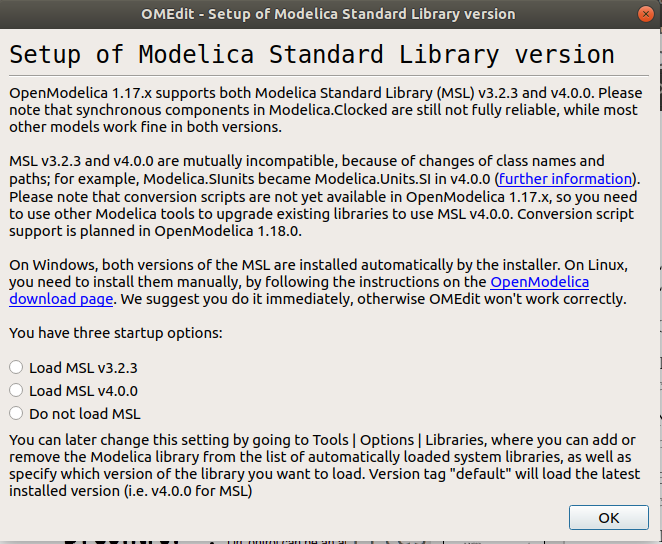
\includegraphics[scale=0.55]{\LocSWfig/OMEdit-libraries.png}
      \caption{Setup of Modelica Standard Library version}
      \label{om-help}
\end{figure}
To know how to execute models in OMEdit, the readers are advised to refer to \secref{OpenModelica-code-execution}. 

\subsection{Simulating models in OpenModelica}\label{OpenModelica-code-execution}
Once you launch OMEdit (either on Windows or on Linux Ubuntu), you should expect a user interface, 
as shown in \figref{om-ui}. In the bottom right of \figref{om-ui}, we can 
see that there are four different tabs - Welcome, Modeling, Plotting, and 
Debugging. In the language of OpenModelica, we refer to these tabs as Perspectives. 
By default, OMEdit gets launched in the Welcome Perspective. We now briefly describe each 
of these Perspectives, as given below:
\begin{enumerate}
      \item Welcome Perspective: It shows the list of recent files and the list of the 
      latest news from {\tt https://www.openmodelica.org}.
      \item Modeling Perpective: It provides the interface where users can 
      create and design their models.
      \item Plotting Perspective: It shows the simulation results of the models. 
      Plotting Perspective will automatically become active 
      when the simulation of the model is finished successfully.
      \item Debugging Perspective: The application automatically switches to Debugging Perspective 
      when the user simulates the class with an algorithmic debugger \cite{om-ref}.
\end{enumerate}

In the left of \figref{om-ui}, there is Libraries Browser below which you can view
the list of libraries loaded in your current session of OMEdit. By default, OMEdit 
comes with a few default libraries, like Modelica, ModelicaReference, etc., as shown in
\figref{om-ui}. These default libraries might not be visible if you have not set up the
Modelica Standard Library version, as given in \figref{om-help}. 
\begin{figure}
      \centering
      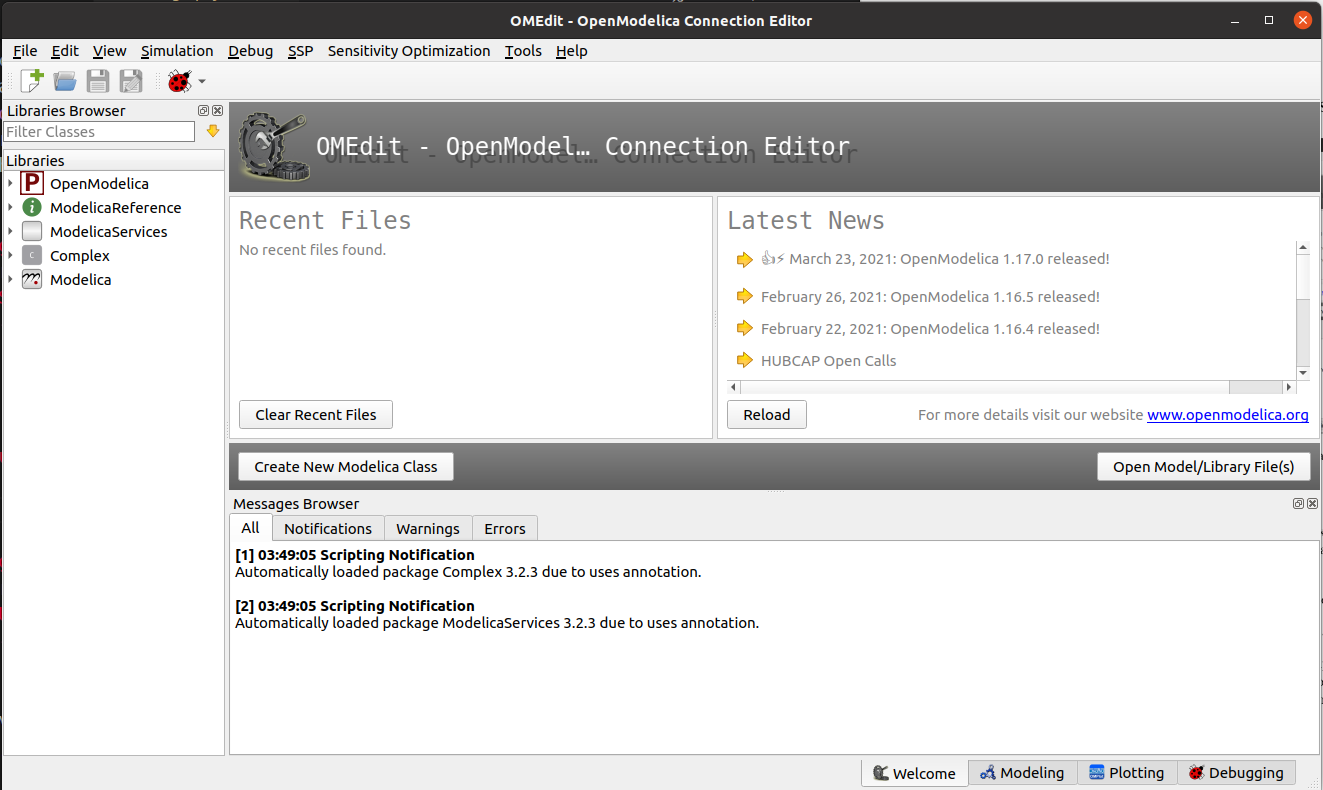
\includegraphics[width=\textwidth]{\LocSWfig/OMEdit-UI.png}
      \caption{User Interface of OMEdit}
      \label{om-ui}
\end{figure}

The files or models in OpenModelica have `.mo' extensions. Though there are several ways to simulate or run 
an OpenModelica model, we will execute the models by utilizing the user interface of OMEdit. To open 
a model in OMEdit, go to the menu bar of OMEdit and click on File -> Open Model/Library File(s), as shown 
in \figref{om-model-open}. Then, select the desired model (with `.mo' extension) and click Open. The names of tabs in
this book have been mentioned according to OpenModelica 1.17.0. You might observe a bit
of difference in these names while working with other versions of OpenModelica. 

\begin{figure}
      \centering
      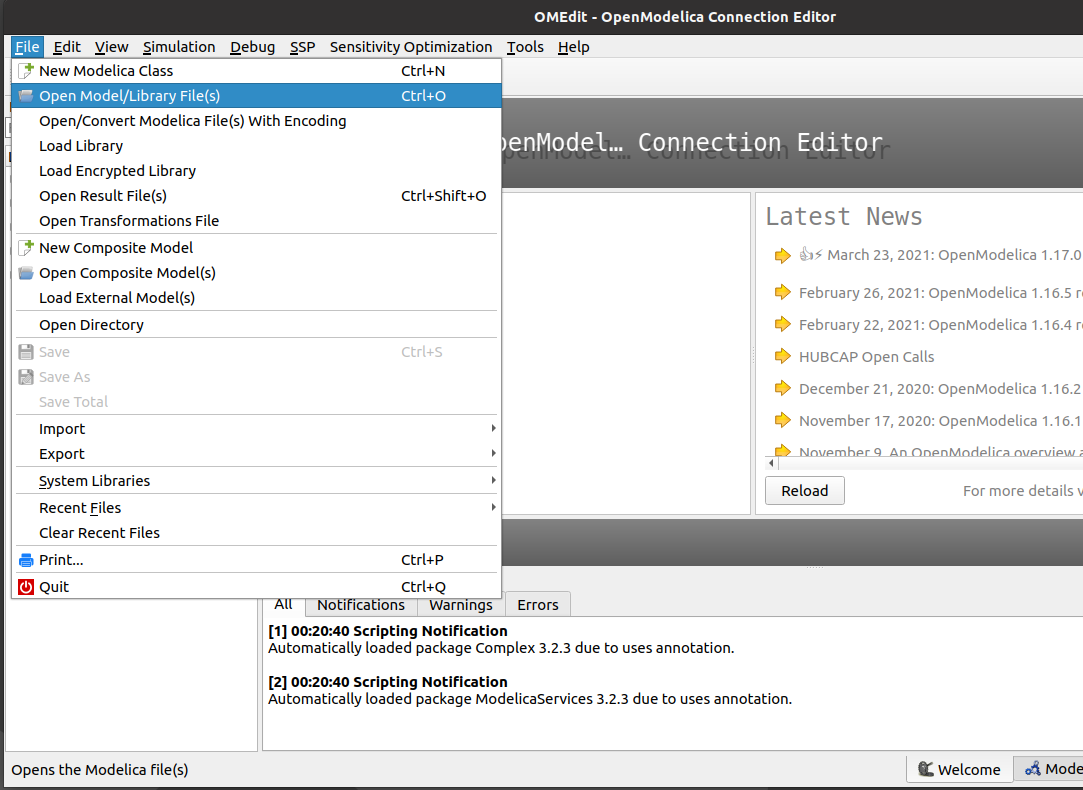
\includegraphics[width=\textwidth]{\LocSWfig/om-open-model.png}
      \caption{Opening a model in OMEdit}
      \label{om-model-open}
\end{figure}

\begin{figure}
      \centering
      \includegraphics[width=\textwidth]{\LocSWfig/om-Modeling.png}
      \caption{Opening a model in diagram view in OMEdit}
      \label{om-modeling}
\end{figure}


\begin{figure}
      \centering
      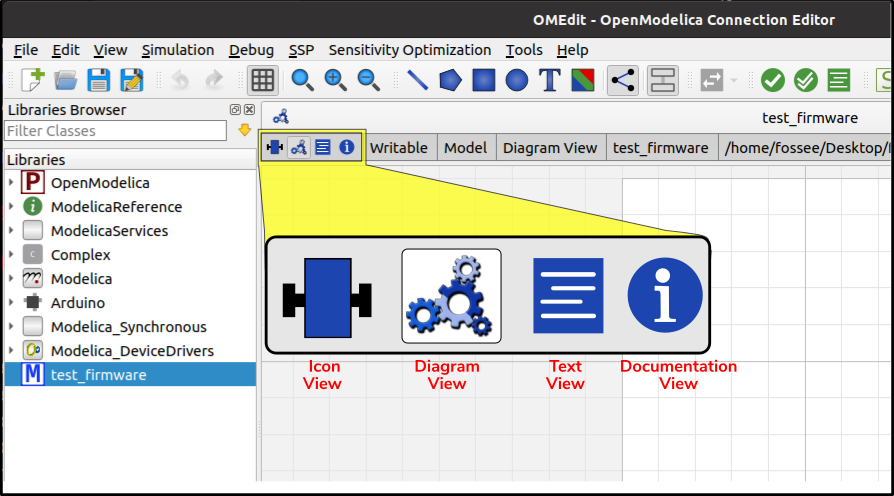
\includegraphics[width=\textwidth]{\LocSWfig/om-modeling-views.png}
      \caption{Different views of a model in OMEdit}
      \label{om-views}
\end{figure}


\begin{figure}
      \centering
      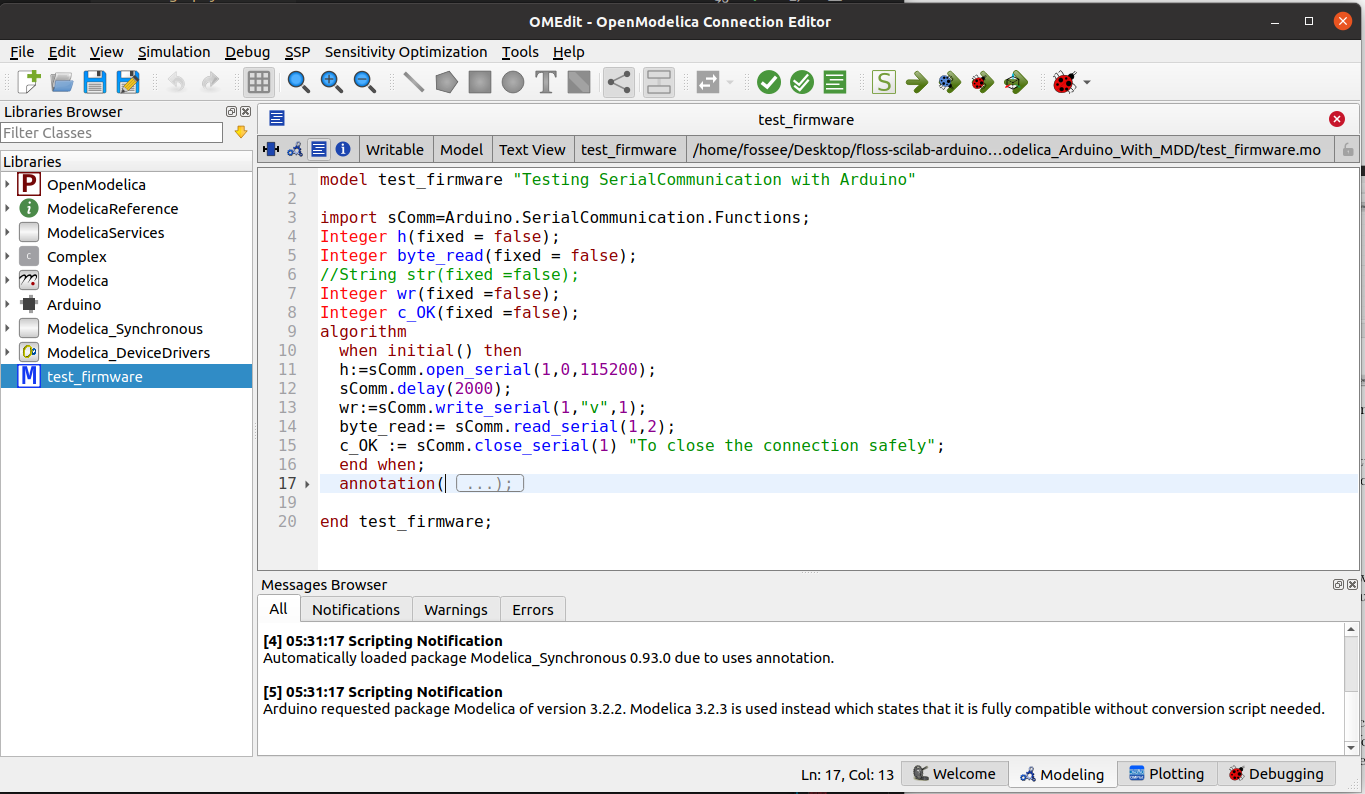
\includegraphics[width=\textwidth]{\LocSWfig/om-text-view.png}
      \caption{Opening a model in text view in OMEdit}
      \label{om-text-view}
\end{figure}

Once you have opened the model in OMEdit, that model should appear under the Libraries
browser, as shown in \figref{om-ui}. To view or simulate that model, you need to 
double-click on the model. It will open the model in Modeling perspective with a Diagram View, as shown 
in the \figref{om-modeling}. In this perspective, there are four different views of 
a model: Icon View, Diagram View, Text View, and Documentation View. All these views have been highlighted in \figref{om-views}. 
By default, OMEdit opens any model in Diagram View. Hence, the models 
having code in text format won't be visible by default in Modeling 
Perspective. To see the code in text format, we need to open the model in 
Text View. For our experiments, we will use Text view mainly. To view the code written for this model, 
we need to click on Text View, as shown in \figref{om-views}. In Text view, the code is now visible, as 
shown in \figref{om-text-view}. Now, one can modify the model as per the requirements. 

Now, we will see how to simulate this model. For this, we need to ensure that OMEdit 
is in Modeling Perspective. Next, we will click on the green right-sided arrow, named as 
Simulate, as shown in \figref{om-simulate}. When we click on Simulate, OMEdit will first 
compile the model and then, it will simulate the model for the time specified in the model itself. 
As OMEdit provides an elegant user interface for simulating the models, 
it will open an output window the moment you click on Simulate. \figref{om-sim-success}
shows the output window after the simulation of our model is finished. Also, we can
observe that the OMEdit is now in Plotting Perspective. 


\begin{figure}
      \centering
      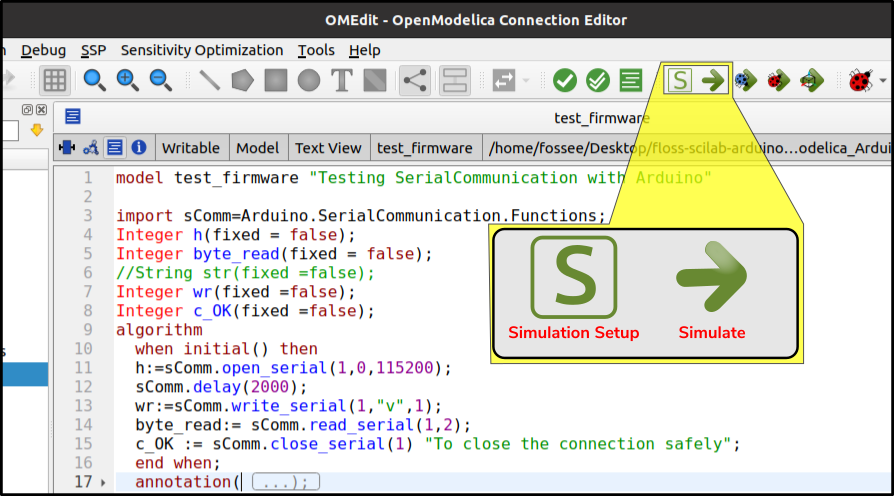
\includegraphics[width=\textwidth]{\LocSWfig/om-simulate.png}
      \caption{Simulating a model in OMEdit}
      \label{om-simulate}
\end{figure}

\begin{figure}
      \centering
      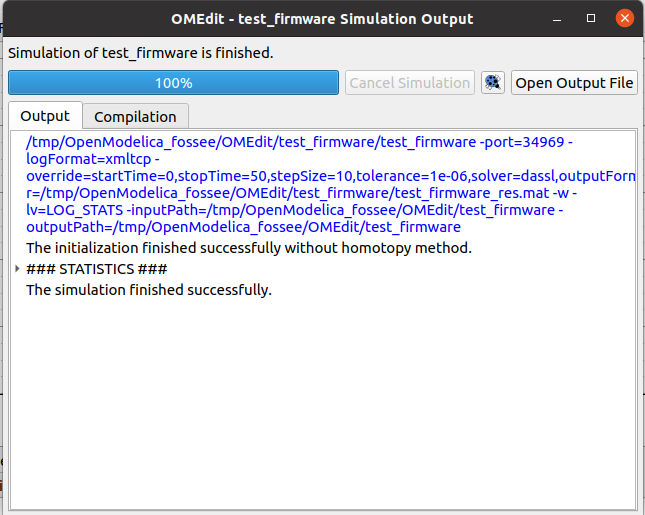
\includegraphics[width=\textwidth]{\LocSWfig/om-sim-success.png}
      \caption{Output window of OMEdit}
      \label{om-sim-success}
\end{figure}

As shown in \figref{om-sim-success}, OMEdit displays the message that "The 
Simulation finished successfully". Had there been any error in simulating the model, 
we would not have received this message. 


\subsection{OpenModelica-Arduino toolbox}\label{sec:load-om-toolbox}
OpenModelica, by default, does not have the capability to connect to Arduino. 
All such add-on functionalities are added to OpenModelica using toolboxes.  
OpenModelica-Arduino toolbox can be found inside {\tt Origin/tools/\\openmodelica/windows} or {\tt Origin/tools/openmodelica/linux} directory,
see \fnrefp{fn:file-loc}.  Use the one depending upon
which operating system you are using. The OpenModelica codes for various
experiments mentioned throughout this book can be found in {\tt Origin/user-code} directory. The {\tt user-code} directory will have
many sub-directories as per the experiments. 

Let us now see how to load OpenModelica-Arduino toolbox. 
\begin{enumerate}
      \item First launch OMEdit. On a Windows system, one may start/launch
            OMEdit from the Start menu. On a Linux system, one has to
            start OMEdit through a terminal, as
            explained in section \ref{openmodelica-install-linux}.
      \item After launching, we have to load OpenModelica-Arduino
            toolbox. To do so, go to the menu bar of OMEdit. 
            Click on {\tt File} and then click on
            the {\tt Open Model/Library File(s)} option as shown in \figref{om-model-open}.
      \item Navigate to {\tt Origin/tools/openmodelica/windows} or {\tt Origin/tools/\\openmodelica/linux}, as the case maybe.
            Select {\tt Arduino.mo} and \\{\tt test\_firmware.mo}, and click Open. The toolbox should now be loaded and available for use. 
      \item \label{itm:library} We will check whether the toolbox has been loaded successfully or not. 
            In OMEdit, under Libraries Browser, look for three new libraries: Arduino,
            Modelica\_Synchronous, Modelica\_DeviceDrivers, and one model test\_firmware.mo. 
            If you are able to view these files, it means that OpenModelica-Arduino toolbox has been loaded successfully. 
            Please note that each time you launch OMEdit, you need to load this toolbox for
            performing the experiments. 
      % \item The {\tt test\_firmware.mo} in the step \ref{itm:library} is the same file which has been mentioned in \secref{om-firmware}.
            % While following \secref{om-firmware}, the readers are advised to execute (or simulate) this file (or model). 
      \item \label{itm:locate} Now, we will locate the models for running the experiments in the upcoming chapters. 
            Under Libraries Browser, click on the arrow before Arduino to see the 
            contents inside this package. Next go to SerialCommunication -> Examples. 
            Under Examples, you will find the list of experiments like led, push, etc., 
            as shown in \figref{om-examples-toolbox}.
      \item \label{itm:simulate} For running the experiments of a particular chapter, click on the corresponding 
            experiment's name. Subsequently, you will find a list of experiments which you can 
            simulate one by one, as explained in \secref{OpenModelica-code-execution}.
      \item For each of the experiments using OpenModelica given in the upcoming chapters, the readers 
            are advised to locate the corresponding model by following the steps
            numbered \ref{itm:locate} and \ref{itm:simulate} and simulate it.  
\end{enumerate}



\begin{figure}
      \centering
      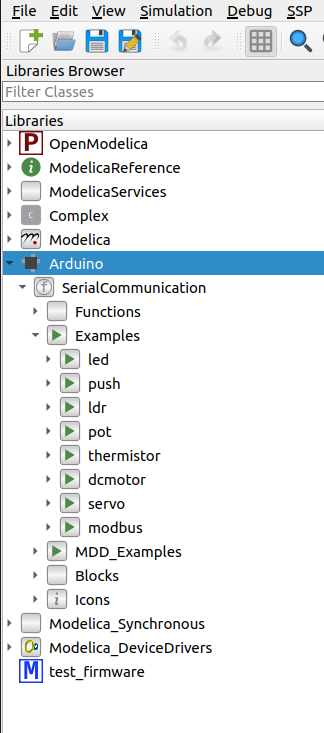
\includegraphics[width=\smfig]{\LocSWfig/om-toolbox-loaded.png}
      \caption{Examples provided in OpenModelica-Arduino toolbox}
      \label{om-examples-toolbox}
\end{figure}

%%%%%begin OpenModelica code

\subsection{Firmware}\label{om-firmware}
\lstset{style=mystyle}
\label{sec:test-firmware-OpenModelica}
\addtocontents{cod}{\protect\addvspace{\codclr}}
We have provided an OpenModelica code/model to check whether the firmware has been
properly installed.  That code/model is listed below. Please ensure that 
you have uploaded the FLOSS firmware given 
in \ardref{ard:firmware} on the \arduino\ board.


\begin{OpenModelicacode}
      \mcaption{An OpenModelica code/model to check whether the firmware is properly installed
            or not}{An OpenModelica code/model to check whether the firmware is properly installed
            or not.  Available at \LocFIMOpenModelicabrief{test\_firmware.mo}. Locate this file 
            inside OpenModelica-Arduino toolbox, as explained in \secref{sec:load-om-toolbox}. Simulate this code/model by following the steps 
            given in  \secref{OpenModelica-code-execution}. If the simulation is
            successful, you should expect an output window in OMEdit as shown in 
            \figref{om-sim-success}.}
      \label{OpenModelica:test-firmware}
      \lstinputlisting{\LocFIMOpenModelicacode/test_firmware.mo}
\end{OpenModelicacode}
